\section*{Problem 6}

The DTFT for an 6 point signal, $x[n]$, 
is shown below. Indicate on the plot the values of the DFT.

\begin{figure}[H]
\caption*{}
\centering
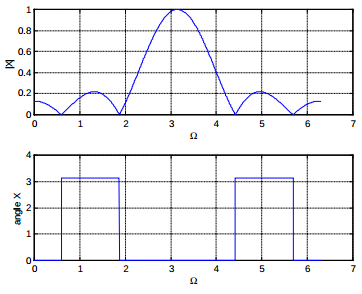
\includegraphics[width=0.5\textwidth]{figs/c4p6.png}
\label{fig:c4p6}
\end{figure} 

\subsection*{Solution}

\begin{equation*}
\begin{aligned}
N &= 6 \\
k &= \left(
\begin{array}{c c c}
 0& 1\cdots & N-1
 \end{array} \right) \\
\omega &= \frac{2 \pi k}{N} \\ 
	   &= \left(
	   \begin{array}{*6c}
	    0 & \frac{\pi}{3} & \frac{2 \pi}{3}\ &\pi& \frac{4 \pi}{3} &\frac{5 \pi}{3}
		\end{array}
		\right) 
\end{aligned}
\end{equation*} 

\begin{figure}[H]
\caption{Values of discrete frecuency}
\centering
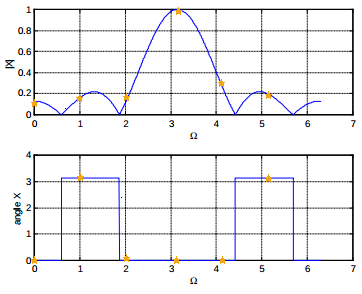
\includegraphics[width=0.5\textwidth]{figs/c4p61.png}
\label{fig:c4p61}
\end{figure} 

